% ============================================================
%  Kapitel 4 — Auswertung
% ============================================================
\section{Auswertung}
\label{sec:auswertung}

\subsection{Magnetisches Phasendiagramm $B_c(T)$ des Bleifilms}

\subsubsection*{Spannungstransitionen $U(B)$}

Abbildung~\ref{fig:vb_curves} zeigt die gemessenen Spannungskurven $U(B)$ des Bleifilms bei 16 verschiedenen Temperaturen zwischen $T = 5{,}82~\mathrm{K}$ und $T = 7{,}20~\mathrm{K}$.
Das Magnetfeld wurde dabei gemäß Gleichung~\eqref{eq:b_recon} aus der Messzeit rekonstruiert.

Im supraleitenden Zustand beträgt die gemessene Spannung $U_\mathrm{SC} \approx 290~\mu\mathrm{V}$, was einem Restwiderstands-Offset aus Zuleitungs- und Kontaktwiderständen entspricht.
Im normalleitenden Zustand liegt die Spannung bei $U_N \approx 7{,}1~\mathrm{mV}$, entsprechend einem Filmwiderstand von $R_N = U_N / I_\mathrm{mess} = 7{,}1~\mathrm{mV} / 100~\mu\mathrm{A} \approx 71~\Omega$.

Für Temperaturen $T \geq 6{,}796~\mathrm{K}$ ist der Film bereits bei $B = 0$ normalleitend; die Filmtemperatur liegt damit über der Null-Feld-Sprungtemperatur des Films.
Bei $T = 5{,}821~\mathrm{K}$ bleibt der Film innerhalb des gesamten Messbereichs ($B_\mathrm{max} \approx 505~\mathrm{mT}$) supraleitend; das kritische Feld liegt damit oberhalb dieser Grenze.

Das kritische Feld $B_c$ wird bei jeder Temperatur als diejenige Feldstärke bestimmt, bei der die Spannung die 50\%-Schwelle
\begin{equation}
    U_{50\%} = \tfrac{1}{2}(U_\mathrm{SC} + U_N)
    \label{eq:uc50}
\end{equation}
überschreitet.
Durch lineare Interpolation zwischen den angrenzenden Datenpunkten ergibt sich eine Genauigkeit von $\Delta B_c \lesssim 5~\mathrm{mT}$.

\begin{figure}[htbp]
    \centering
    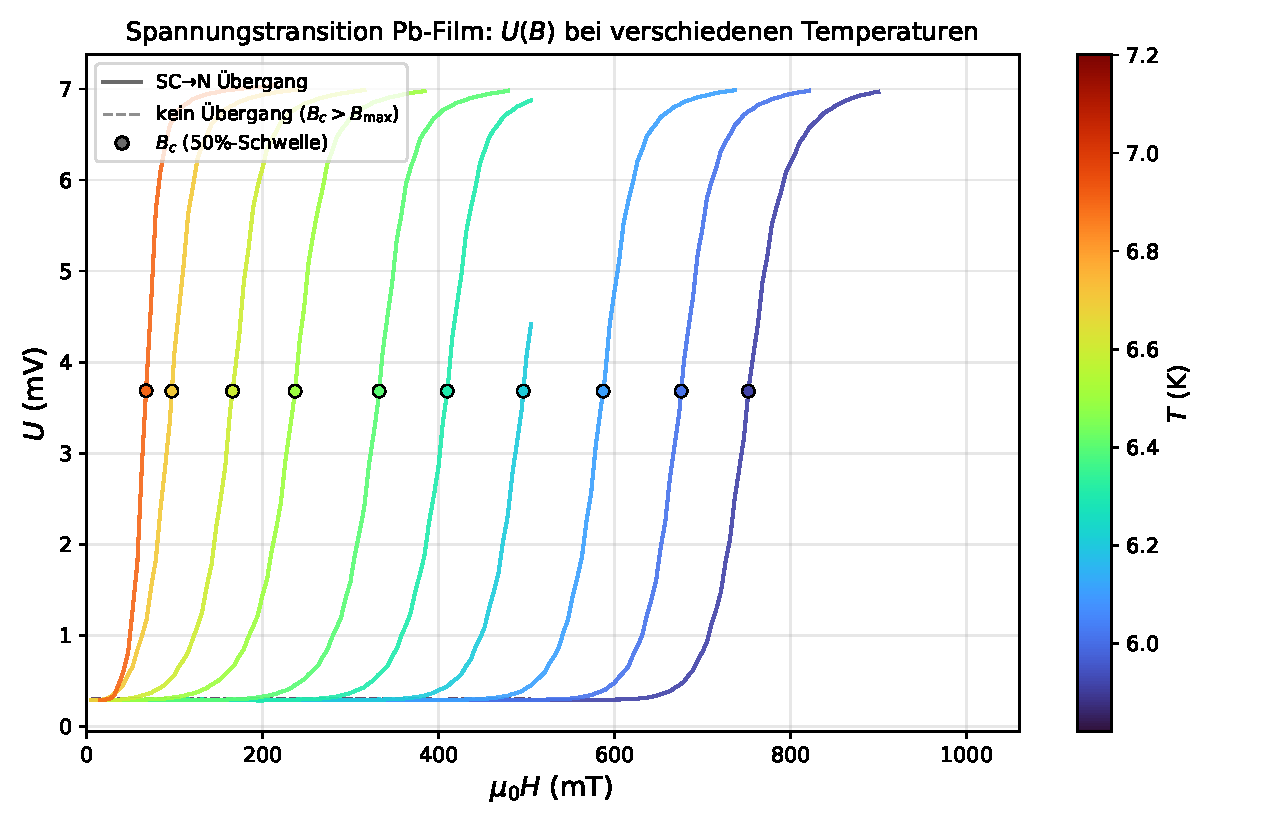
\includegraphics[width=0.9\linewidth]{../figures/fig_vb_curves.pdf}
    \caption{Spannungstransition $U(B)$ des Bleifilms bei verschiedenen Temperaturen
    (Farbkodierung: blau $= 5{,}82~\mathrm{K}$, rot $= 7{,}20~\mathrm{K}$).
    Durchgehende Linien: klarer SC-$\to$N-Übergang.
    Gepunktete Linien: kein Übergang im Messbereich oder Film bereits normal bei $B=0$.
    Kreissymbole markieren die extrahierten $B_c$-Werte (50\%-Schwelle).}
    \label{fig:vb_curves}
\end{figure}

\subsubsection*{Parabolisches Phasendiagramm}

Abbildung~\ref{fig:bc_phase} zeigt die so bestimmten $B_c(T)$-Werte zusammen mit dem Fit des parabolischen Gesetzes~\eqref{eq:bc_parabola}.
Insgesamt liegen 9 auswertbare Punkte im Temperaturbereich $5{,}916~\mathrm{K} \leq T \leq 6{,}901~\mathrm{K}$ vor; ein zusätzlicher Punkt bei $T = 5{,}821~\mathrm{K}$ liefert nur eine untere Schranke $B_c > 505~\mathrm{mT}$.

Die Anpassung von Gleichung~\eqref{eq:bc_parabola} an die 10 Messpunkte mit freien Parametern $B_c(0)$ und $T_c$ ergibt:
\begin{align}
    B_c(0) &= (2779 \pm 165)~\mathrm{mT}, \label{eq:fit_bc0} \\
    T_c     &= (6{,}861 \pm 0{,}038)~\mathrm{K}. \label{eq:fit_tc}
\end{align}
Die parabolische Form wird durch die Daten gut bestätigt (vgl.\ Abbildung~\ref{fig:bc_phase}).

\begin{figure}[htbp]
    \centering
    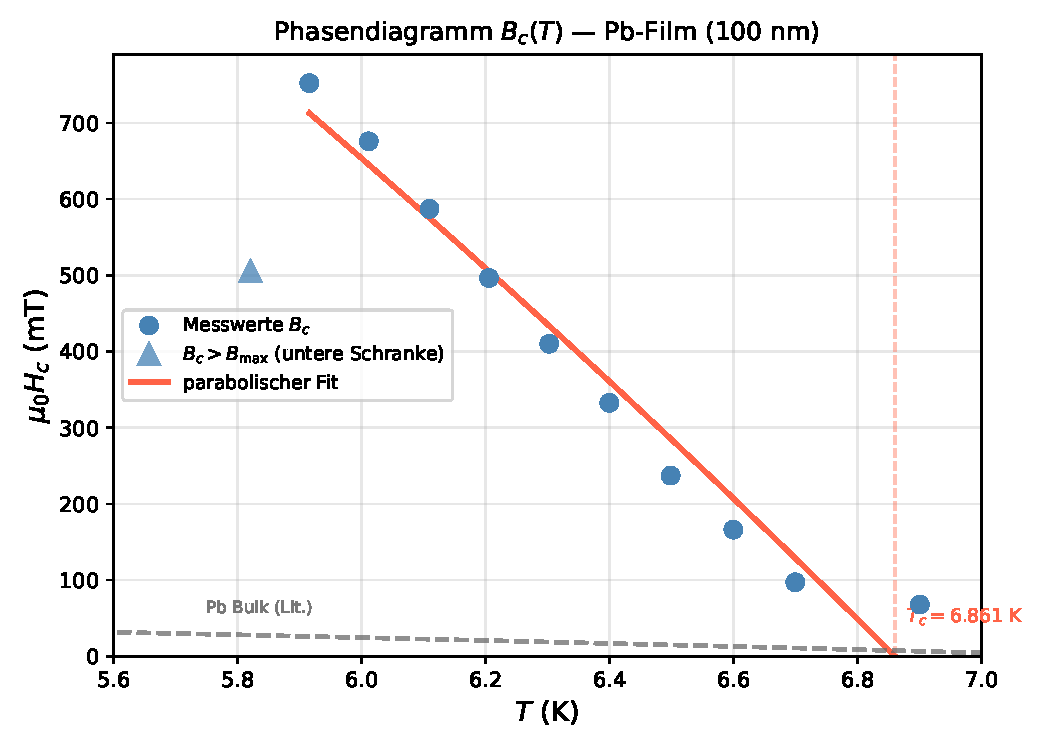
\includegraphics[width=0.88\linewidth]{../figures/fig_bc_phase.pdf}
    \caption{Magnetisches Phasendiagramm $B_c(T)$ des Pb-Films (100~nm).
    Kreise: auswertbare Messpunkte.
    Dreieck: untere Schranke bei $T = 5{,}82~\mathrm{K}$ ($B_c > 505~\mathrm{mT}$).
    Rote Kurve: parabolischer Fit~\eqref{eq:bc_parabola} mit $B_c(0) = 2779~\mathrm{mT}$, $T_c = 6{,}861~\mathrm{K}$.
    Gestrichelte schwarze Kurve: Pb-Bulk-Literaturwerte ($B_c(0) = 80~\mathrm{mT}$, $T_c = 7{,}2~\mathrm{K}$).}
    \label{fig:bc_phase}
\end{figure}

\subsection{Kritischer Strom $I_c(T)$}

\subsubsection*{I-V-Kennlinien}

Abbildung~\ref{fig:iv_curves} zeigt die gemessenen I-V-Kennlinien des Bleifilms bei acht Temperaturen zwischen $T = 6{,}499~\mathrm{K}$ und $T = 6{,}800~\mathrm{K}$.
Aufgetragen ist die Filmspannung abzüglich der SC-Basislinie ($U_0 \approx 290~\mu\mathrm{V}$) über dem Strom.
Bis zum kritischen Strom $I_c$ bleibt $\Delta U \approx 0$; darüber wächst $\Delta U$ steil an und geht in einen nahezu linearen Verlauf über, der dem Normalzustand entspricht.

\begin{figure}[htbp]
    \centering
    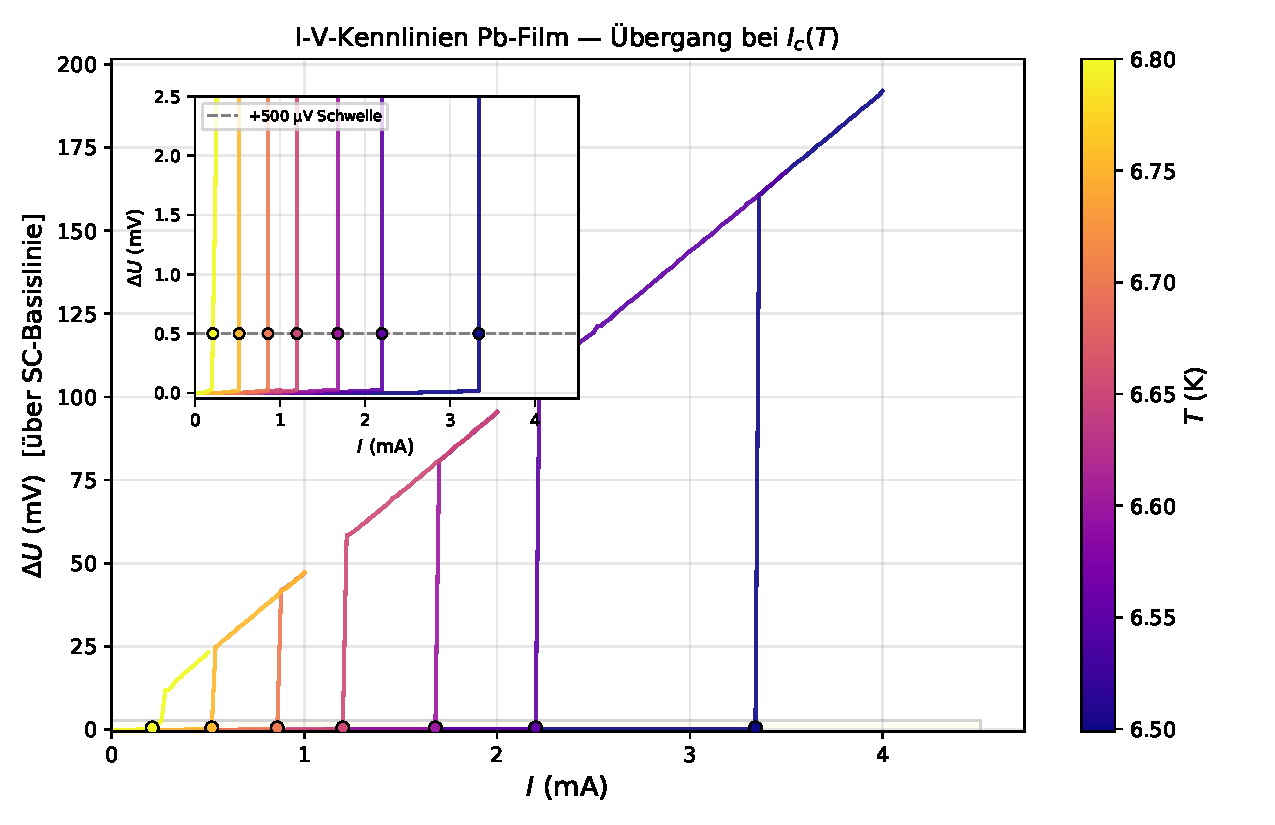
\includegraphics[width=0.9\linewidth]{../figures/fig_iv_curves.pdf}
    \caption{I-V-Kennlinien des Pb-Films bei verschiedenen Temperaturen
    (Farbkodierung: lila $= 6{,}499~\mathrm{K}$, gelb $= 6{,}800~\mathrm{K}$).
    Aufgetragen ist $\Delta U = U - U_0$ mit SC-Basislinie $U_0 \approx 290~\mu\mathrm{V}$.
    Kreissymbole: extrahierte $I_c$-Werte (Schwelle $\Delta U > 500~\mu\mathrm{V}$).}
    \label{fig:iv_curves}
\end{figure}

\subsubsection*{Temperaturabhängigkeit von $I_c$}

Abbildung~\ref{fig:ic_temp} zeigt die extrahierten $I_c(T)$-Werte.
Mit steigender Temperatur nimmt $I_c$ monoton ab.
Bei $T = 6{,}499~\mathrm{K}$ beträgt $I_c \approx 3{,}34~\mathrm{mA}$, bei $T = 6{,}800~\mathrm{K}$ nur noch $I_c \approx 212~\mu\mathrm{A}$.
Bei der Messung bei $T = 6{,}650~\mathrm{K}$ wurde der Strom nur bis $1~\mathrm{mA}$ erhöht, ohne dass ein Übergang eintrat; dieser Punkt liefert daher nur eine untere Schranke $I_c > 1~\mathrm{mA}$.

Unter Verwendung des aus dem $B_c(T)$-Fit bestimmten $T_c = 6{,}861~\mathrm{K}$ wird das Potenzgesetz
\begin{equation}
    I_c(T) = I_c(0)\left(1 - \frac{T}{T_c}\right)^n
    \label{eq:ic_fit}
\end{equation}
an die Daten angepasst (mit festgehaltenem $T_c$).
Dies liefert den Exponenten $n = 1{,}75 \pm 0{,}16$, konsistent mit dem theoretischen Ginzburg-Landau-Wert $n = 3/2$ für den Grenzfall nahe $T_c$.

\begin{figure}[htbp]
    \centering
    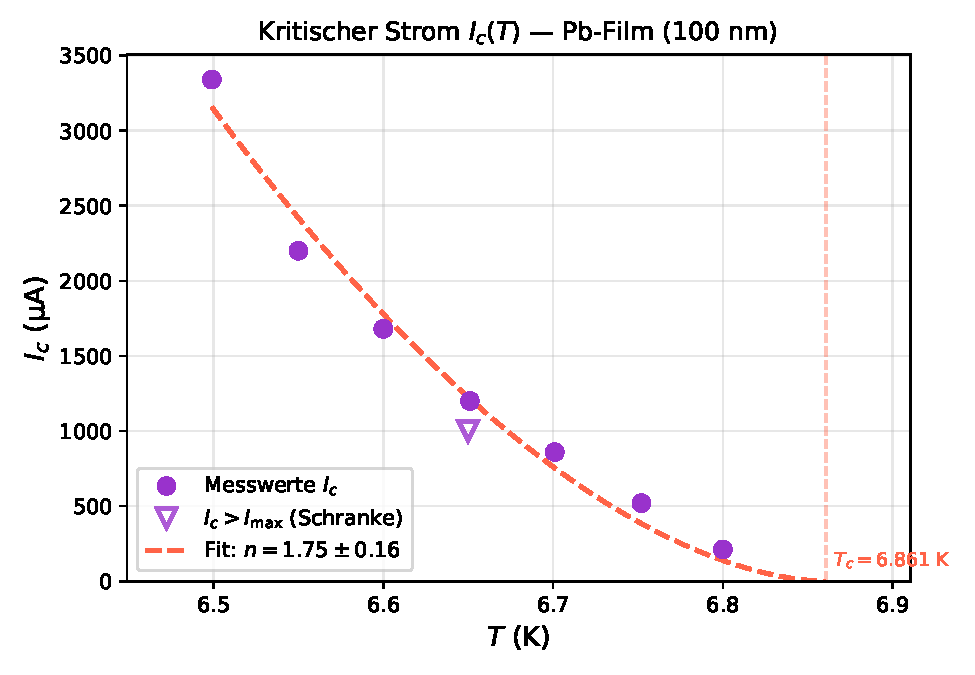
\includegraphics[width=0.82\linewidth]{../figures/fig_ic_temp.pdf}
    \caption{Kritischer Strom $I_c(T)$ des Pb-Films (100~nm).
    Kreise: Messwerte.
    Dreieck: untere Schranke bei $T = 6{,}650~\mathrm{K}$.
    Gestrichelte Kurve: Fit~\eqref{eq:ic_fit} mit festgehaltenem $T_c = 6{,}861~\mathrm{K}$ (aus $B_c(T)$-Fit) und $n = 1{,}75$.}
    \label{fig:ic_temp}
\end{figure}

\subsection{Levitation (qualitativ)}

Im Rahmen einer qualitativen Demonstration wurde ein Neodym-Permanentmagnet über eine gekühlte YBCO-Tablette gehalten und in mehreren Zentimetern Abstand zur Oberfläche frei schwebend beobachtet.
Das Experiment wurde sowohl im Zero-Field-Cooling- als auch im Field-Cooling-Modus durchgeführt.
Im Zero-Field-Cooling-Modus levitierte der Magnet stabil; im Field-Cooling-Modus war zwar die Levitation geringer, jedoch zeigte die Tablette deutliches Flux-Pinning: Der Magnet konnte innerhalb eines gewissen Bereichs lateral bewegt werden, ohne dass er herunterfiel.
Eine quantitative Auswertung (z.\,B.\ Levitationshöhe, Haltekraft) wurde nicht vorgenommen.
